\documentclass[11pt,letterpaper]{article}

\usepackage[margin=1in]{geometry}
\usepackage[utf8]{inputenc}
\usepackage[T1]{fontenc}
\usepackage{lmodern}
\usepackage{microtype}
\usepackage{amssymb}
\usepackage{enumitem}
\usepackage{hyperref}
\usepackage{xcolor}
\usepackage{listings}
\usepackage{fancyhdr}
\usepackage{titlesec}
\usepackage{tikz}
\usetikzlibrary{shapes.geometric, shapes.multipart, positioning, arrows.meta, calc}
\usepackage{float}

\hypersetup{colorlinks=true,linkcolor=black,urlcolor=blue!60!black}

\setlength{\headheight}{14pt}
\pagestyle{fancy}
\fancyhf{}
\fancyhead[L]{CS6083 --- Project \#1 (snickr)}
\fancyhead[R]{Spring 2026}
\fancyfoot[C]{\thepage}
\emergencystretch=2em

\titlespacing*{\section}{0pt}{1em}{0.4em}

% SQL listings
\definecolor{sqlkw}{RGB}{0,0,180}
\definecolor{sqlstr}{RGB}{163,21,21}
\definecolor{sqlcmt}{RGB}{0,120,0}
\definecolor{sqlbg}{RGB}{248,248,248}
\lstdefinestyle{sql}{
  language=SQL, basicstyle=\ttfamily\small,
  keywordstyle=\color{sqlkw}\bfseries, stringstyle=\color{sqlstr},
  commentstyle=\color{sqlcmt}\itshape, backgroundcolor=\color{sqlbg},
  frame=single, rulecolor=\color{black!20},
  breaklines=true, breakatwhitespace=true, showstringspaces=false,
  tabsize=2, numbers=none, xleftmargin=0.8em,
  morekeywords={ILIKE,RETURNING,BIGSERIAL,TIMESTAMP,TEXT,VARCHAR,BOOLEAN,INTERVAL}
}
\lstset{style=sql}

% Plain ASCII diagram style (no language highlighting)
\lstdefinestyle{ascii}{
  language={},
  basicstyle=\ttfamily\footnotesize,
  keywordstyle={}, commentstyle={}, stringstyle={},
  frame=none, backgroundcolor=\color{white},
  keepspaces=true, columns=fullflexible, breaklines=true,
  showstringspaces=false, numbers=none
}

% Query-result block style
\lstdefinestyle{result}{
  language={},
  basicstyle=\ttfamily\fontsize{6.5}{7.2}\selectfont,
  keywordstyle={}, commentstyle={}, stringstyle={},
  backgroundcolor=\color{sqlbg},
  frame=single, rulecolor=\color{black!20},
  keepspaces=true, columns=fullflexible, breaklines=true,
  breakatwhitespace=false, breakindent=0pt,
  showstringspaces=false, numbers=none, xleftmargin=0em
}

\title{\textbf{snickr: Relational Database Design}\\[0.2em]
       \large CS6083 --- Project \#1}
\author{Shichen Zhang \quad (\texttt{sz4968@nyu.edu})\\
        Zihang Yu \quad (\texttt{zy3493@nyu.edu})}
\date{April 27, 2026}

\begin{document}
\maketitle
\thispagestyle{fancy}

\section*{Introduction}
\emph{snickr} is a Slack-like collaboration system where users create
workspaces, invite members, create public/private/direct channels, and exchange
messages inside those channels. This report presents a relational design for
the system, including the ER model, relational schema, SQL DDL, required
queries, and a small sample dataset used to test the design.

% =======================================================
\section*{(a) Database Schema Design}
% =======================================================

\noindent\textbf{ER diagram.}

\begin{center}
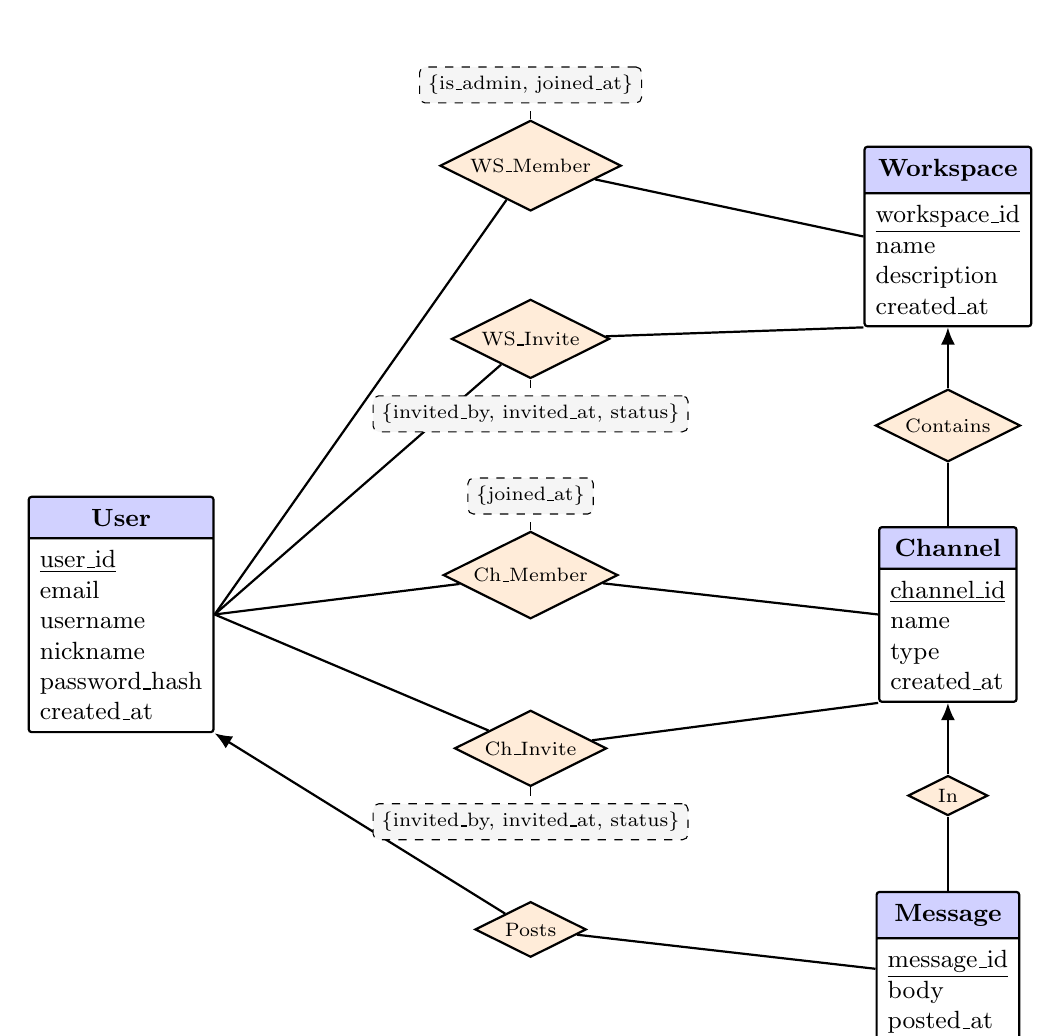
\begin{tikzpicture}[
  every node/.style={font=\small},
  entity/.style={
    rectangle split, rectangle split parts=2,
    draw, thick, rounded corners=1pt,
    rectangle split part fill={blue!18, white},
    inner sep=4pt, align=left,
  },
  rel/.style={
    diamond, draw, thick, aspect=2, inner sep=2pt,
    fill=orange!15, font=\scriptsize,
  },
  attrs/.style={
    rectangle, draw, thin, dashed, rounded corners=2pt,
    fill=gray!8, font=\scriptsize, inner sep=3pt, align=left,
  },
  one/.style={-{Latex[length=2.2mm,width=1.8mm]}, thick},
  mn/.style={thick},
]

% ---- Entities ----
\node[entity] (user) at (0, 0) {%
  \textbf{User}
  \nodepart{second}%
  \underline{user\_id}\\
  email\\
  username\\
  nickname\\
  password\_hash\\
  created\_at
};

\node[entity] (workspace) at (10.5, 4.8) {%
  \textbf{Workspace}
  \nodepart{second}%
  \underline{workspace\_id}\\
  name\\
  description\\
  created\_at
};

\node[entity] (channel) at (10.5, 0) {%
  \textbf{Channel}
  \nodepart{second}%
  \underline{channel\_id}\\
  name\\
  type\\
  created\_at
};

\node[entity] (message) at (10.5, -4.5) {%
  \textbf{Message}
  \nodepart{second}%
  \underline{message\_id}\\
  body\\
  posted\_at
};

% ---- Relationship diamonds ---- (spaced so attr boxes fit between diamonds)
\node[rel] (wsmem) at (5.2, 5.7)   {WS\_Member};
\node[rel] (wsinv) at (5.2, 3.5)   {WS\_Invite};
\node[rel] (chmem) at (5.2, 0.5)   {Ch\_Member};
\node[rel] (chinv) at (5.2, -1.7)  {Ch\_Invite};
\node[rel] (contains) at (10.5, 2.4) {Contains};
\node[rel] (inrel)    at (10.5, -2.3) {In};
\node[rel] (posts)    at (5.2, -4.0) {Posts};

% ---- M:N edges (plain) ----
\draw[mn] (user.east) -- (wsmem) -- (workspace.west);
\draw[mn] (user.east) -- (wsinv) -- (workspace.south west);
\draw[mn] (user.east) -- (chmem) -- (channel.west);
\draw[mn] (user.east) -- (chinv) -- (channel.south west);

% ---- 1:N edges (arrow points to the "1" side) ----
\draw[mn]  (channel.north) -- (contains);
\draw[one] (contains) -- (workspace.south);

\draw[mn]  (message.north) -- (inrel);
\draw[one] (inrel) -- (channel.south);

\draw[mn]  (message.west) -- (posts);
\draw[one] (posts) -- (user.south east);

% ---- Attribute boxes (dashed): all on the "outside", no overlap with edges ----
%  WS_* diamonds: attrs above them
%  Ch_* diamonds: attrs below them
\node[attrs, above=2mm of wsmem] (wsmemA) {\{is\_admin, joined\_at\}};
\draw[dashed] (wsmem.north) -- (wsmemA.south);

\node[attrs, below=2mm of wsinv] (wsinvA) {\{invited\_by, invited\_at, status\}};
\draw[dashed] (wsinv.south) -- (wsinvA.north);

\node[attrs, above=2mm of chmem] (chmemA) {\{joined\_at\}};
\draw[dashed] (chmem.north) -- (chmemA.south);

\node[attrs, below=2mm of chinv] (chinvA) {\{invited\_by, invited\_at, status\}};
\draw[dashed] (chinv.south) -- (chinvA.north);

\end{tikzpicture}
\end{center}

\paragraph{Relational schema.}

\begin{itemize}[leftmargin=1.4em,itemsep=1pt]
  \item \textbf{User}(\underline{user\_id}, email, username, nickname, password\_hash, created\_at)\\
        UNIQUE(email), UNIQUE(username).
  \item \textbf{Workspace}(\underline{workspace\_id}, name, description, created\_by, created\_at)\\
        FK: created\_by $\to$ User(user\_id); UNIQUE(created\_by, name).
  \item \textbf{WorkspaceMember}(\underline{workspace\_id, user\_id}, is\_admin, joined\_at)\\
        FKs: workspace\_id $\to$ Workspace, user\_id $\to$ User.
  \item \textbf{WorkspaceInvitation}(\underline{workspace\_id, invitee\_user\_id}, invited\_by, invited\_at, status)\\
        FKs: workspace\_id $\to$ Workspace; invitee\_user\_id, invited\_by $\to$ User.
  \item \textbf{Channel}(\underline{channel\_id}, workspace\_id, name, type, created\_by, created\_at)\\
        FKs: workspace\_id $\to$ Workspace, created\_by $\to$ User; UNIQUE(workspace\_id, name).
  \item \textbf{ChannelMember}(\underline{channel\_id, user\_id}, joined\_at)\\
        FKs: channel\_id $\to$ Channel, user\_id $\to$ User.
  \item \textbf{ChannelInvitation}(\underline{channel\_id, invitee\_user\_id}, invited\_by, invited\_at, status)\\
        FKs: channel\_id $\to$ Channel; invitee\_user\_id, invited\_by $\to$ User.
  \item \textbf{Message}(\underline{message\_id}, channel\_id, sender\_user\_id, body, posted\_at)\\
        FKs: channel\_id $\to$ Channel, sender\_user\_id $\to$ User.
\end{itemize}

\paragraph{Assumptions.}
Email and username are globally unique; workspace names are unique per creator;
channel names are unique only within a workspace; admin is a boolean on
workspace membership rather than a separate entity; a direct channel is a
channel of type \texttt{direct} with exactly two members (cardinality enforced in
the application); channel invitations are issued only to users who are already
members of the channel's workspace (enforced in the application); timestamps
are stored on every action-bearing row.

\paragraph{Design justification.}
\begin{itemize}[leftmargin=1.4em,itemsep=2pt]
  \item \textbf{One \textbf{Channel} table with a \texttt{type} enum} rather
        than separate tables for public, private, and direct channels. All
        three share the same attributes, so subtyping would add joins without
        adding structure.
  \item \textbf{Admin is a boolean on \textbf{WorkspaceMember}}, not a
        separate entity. Every admin is already a member, so a dedicated
        \textbf{Admin} table would duplicate the membership relationship.
  \item \textbf{Separate membership and invitation tables.} Membership records
        an accepted state with relationship-level attributes
        (\texttt{is\_admin}, \texttt{joined\_at}); invitation records a
        pending state with its own attributes (\texttt{invited\_by},
        \texttt{invited\_at}, \texttt{status}). Mixing them in one table would
        conflate ``joined'' with ``invited but not yet joined''.
  \item \textbf{Separate invitation tables for workspaces and channels.}
        They point at different parents, so keeping them apart lets each
        table declare a clean foreign key.
  \item \textbf{Composite natural keys} \texttt{(workspace\_id, user\_id)} and
        \texttt{(channel\_id, user\_id)} on the four membership / invitation
        tables. No surrogate id is needed and the ``one row per pair''
        invariant is structural rather than an extra \texttt{UNIQUE}
        constraint.
\end{itemize}

\paragraph{Procedures / Application Logic.}
This design does not rely on database stored procedures or triggers. Multi-step
operations are handled by the application using ordinary SQL statements. For
example, creating a public channel first inserts the channel and then inserts
the creator into \texttt{channel\_members} if the first step succeeds. Likewise,
rules such as ``a direct channel has exactly two members'' and ``channel
invitations are issued only to members of the channel's workspace'' are checked
by the application before the corresponding insert operations are executed.

% =======================================================
\section*{(b) SQL Schema (DDL)}
% =======================================================

\begin{lstlisting}
CREATE TABLE users (
    user_id       BIGSERIAL    PRIMARY KEY,
    email         VARCHAR(255) NOT NULL UNIQUE,
    username      VARCHAR(64)  NOT NULL UNIQUE,
    nickname      VARCHAR(64)  NOT NULL,
    password_hash VARCHAR(255) NOT NULL,
    created_at    TIMESTAMP    NOT NULL DEFAULT CURRENT_TIMESTAMP
);

CREATE TABLE workspaces (
    workspace_id BIGSERIAL    PRIMARY KEY,
    name         VARCHAR(128) NOT NULL,
    description  TEXT,
    created_by   BIGINT       NOT NULL REFERENCES users(user_id),
    created_at   TIMESTAMP    NOT NULL DEFAULT CURRENT_TIMESTAMP,
    UNIQUE (created_by, name)
);

CREATE TABLE workspace_members (
    workspace_id BIGINT    NOT NULL REFERENCES workspaces(workspace_id),
    user_id      BIGINT    NOT NULL REFERENCES users(user_id),
    is_admin     BOOLEAN   NOT NULL DEFAULT FALSE,
    joined_at    TIMESTAMP NOT NULL DEFAULT CURRENT_TIMESTAMP,
    PRIMARY KEY (workspace_id, user_id)
);

CREATE TABLE workspace_invitations (
    workspace_id    BIGINT    NOT NULL REFERENCES workspaces(workspace_id),
    invitee_user_id BIGINT    NOT NULL REFERENCES users(user_id),
    invited_by      BIGINT    NOT NULL REFERENCES users(user_id),
    invited_at      TIMESTAMP NOT NULL DEFAULT CURRENT_TIMESTAMP,
    status          VARCHAR(16) NOT NULL DEFAULT 'pending'
                    CHECK (status IN ('pending','accepted','declined')),
    PRIMARY KEY (workspace_id, invitee_user_id)
);

CREATE TABLE channels (
    channel_id   BIGSERIAL    PRIMARY KEY,
    workspace_id BIGINT       NOT NULL REFERENCES workspaces(workspace_id),
    name         VARCHAR(128) NOT NULL,
    type         VARCHAR(16)  NOT NULL
                 CHECK (type IN ('public','private','direct')),
    created_by   BIGINT       NOT NULL REFERENCES users(user_id),
    created_at   TIMESTAMP    NOT NULL DEFAULT CURRENT_TIMESTAMP,
    UNIQUE (workspace_id, name)
);

CREATE TABLE channel_members (
    channel_id BIGINT    NOT NULL REFERENCES channels(channel_id),
    user_id    BIGINT    NOT NULL REFERENCES users(user_id),
    joined_at  TIMESTAMP NOT NULL DEFAULT CURRENT_TIMESTAMP,
    PRIMARY KEY (channel_id, user_id)
);

CREATE TABLE channel_invitations (
    channel_id      BIGINT    NOT NULL REFERENCES channels(channel_id),
    invitee_user_id BIGINT    NOT NULL REFERENCES users(user_id),
    invited_by      BIGINT    NOT NULL REFERENCES users(user_id),
    invited_at      TIMESTAMP NOT NULL DEFAULT CURRENT_TIMESTAMP,
    status          VARCHAR(16) NOT NULL DEFAULT 'pending'
                    CHECK (status IN ('pending','accepted','declined')),
    PRIMARY KEY (channel_id, invitee_user_id)
);

CREATE TABLE messages (
    message_id     BIGSERIAL PRIMARY KEY,
    channel_id     BIGINT    NOT NULL REFERENCES channels(channel_id),
    sender_user_id BIGINT    NOT NULL REFERENCES users(user_id),
    body           TEXT      NOT NULL,
    posted_at      TIMESTAMP NOT NULL DEFAULT CURRENT_TIMESTAMP
);

CREATE INDEX idx_messages_channel_time ON messages(channel_id, posted_at);
CREATE INDEX idx_messages_sender       ON messages(sender_user_id);
\end{lstlisting}

% =======================================================
\section*{(c) Required SQL Queries}
% =======================================================

\subsection*{(1) Create a new user account}
\begin{lstlisting}
INSERT INTO users (email, username, nickname, password_hash)
VALUES (:email, :username, :nickname, :password_hash)
RETURNING user_id;
\end{lstlisting}

\subsection*{(2) Create a public channel (with authorization check)}
\begin{lstlisting}
INSERT INTO channels (workspace_id, name, type, created_by)
SELECT :workspace_id, :name, 'public', :user_id
WHERE EXISTS (
    SELECT 1 FROM workspace_members
    WHERE workspace_id = :workspace_id AND user_id = :user_id
)
RETURNING channel_id;

INSERT INTO channel_members (channel_id, user_id)
VALUES (:new_channel_id, :user_id);
\end{lstlisting}
Here \texttt{:new\_channel\_id} is the \texttt{channel\_id} returned by the
first insert. The second insert is executed by the application only if the
first insert returns a \texttt{channel\_id}.

\subsection*{(3) For each workspace, list all administrators}
\begin{lstlisting}
SELECT w.workspace_id, w.name AS workspace, u.username AS administrator
FROM   workspaces w
JOIN   workspace_members wm ON wm.workspace_id = w.workspace_id
JOIN   users u              ON u.user_id       = wm.user_id
WHERE  wm.is_admin = TRUE
ORDER BY w.workspace_id, u.username;
\end{lstlisting}

\subsection*{(4) Per public channel: \# invitees invited $>$5 days ago, not yet joined}
\begin{lstlisting}
SELECT c.channel_id, c.name,
       COUNT(ci.invitee_user_id) FILTER (WHERE cm.user_id IS NULL)
       AS stale_unjoined_invites
FROM   channels c
LEFT   JOIN channel_invitations ci
       ON ci.channel_id = c.channel_id
      AND ci.invited_at < CURRENT_TIMESTAMP - INTERVAL '5 days'
LEFT   JOIN channel_members cm
       ON cm.channel_id = ci.channel_id AND cm.user_id = ci.invitee_user_id
WHERE  c.workspace_id = :workspace_id
  AND  c.type = 'public'
GROUP BY c.channel_id, c.name
ORDER BY c.name;
\end{lstlisting}

\subsection*{(5) All messages in a channel, chronological order}
\begin{lstlisting}
SELECT m.message_id, m.posted_at, u.username, m.body
FROM   messages m
JOIN   users u ON u.user_id = m.sender_user_id
WHERE  m.channel_id = :channel_id
ORDER BY m.posted_at ASC, m.message_id ASC;
\end{lstlisting}

\subsection*{(6) All messages posted by a given user}
\begin{lstlisting}
SELECT m.message_id, w.name AS workspace, c.name AS channel,
       m.posted_at, m.body
FROM   messages m
JOIN   channels   c ON c.channel_id   = m.channel_id
JOIN   workspaces w ON w.workspace_id = c.workspace_id
WHERE  m.sender_user_id = :user_id
ORDER BY m.posted_at DESC;
\end{lstlisting}

\subsection*{(7) Accessible messages containing ``perpendicular''}
\begin{lstlisting}
SELECT m.message_id, w.name AS workspace, c.name AS channel,
       u.username AS author, m.posted_at, m.body
FROM   messages m
JOIN   channels         c  ON c.channel_id    = m.channel_id
JOIN   workspaces       w  ON w.workspace_id  = c.workspace_id
JOIN   users            u  ON u.user_id       = m.sender_user_id
JOIN   channel_members  cm ON cm.channel_id   = c.channel_id
                          AND cm.user_id      = :user_id
JOIN   workspace_members wm ON wm.workspace_id = w.workspace_id
                           AND wm.user_id      = :user_id
WHERE  m.body ILIKE '%perpendicular%'
ORDER BY m.posted_at DESC;
\end{lstlisting}

% =======================================================
\section*{(d) Sample Data and Testing}
% =======================================================

\subsection*{Sample Data}

The sample data populates 6 users, 2 workspaces, 5 channels, 13 messages, and
3 pending invitations. The diagram below summarizes the data as a small
workspace map. Alice, Bob, Carol, Dave, Eve, and Frank are the users; asterisks
mark users who are administrators in at least one workspace. The first
workspace, Acme Co., has Alice and Bob as admins and Carol and Dave as regular
members. It contains a public \texttt{\#general} channel, a private
\texttt{\#hiring} channel, and a direct channel between Alice and Carol. Dave is
listed as an Acme workspace member but is intentionally not a member of any
Acme channel.

The second workspace, Coop Board, has Eve as admin and Frank and Alice as
regular members, so Alice appears in both workspaces. Coop Board contains a
public \texttt{\#announcements} channel and a private \texttt{\#finance}
channel. The message counts are shown inside each channel box, and channels
include notes about whether any message contains the word ``perpendicular''.
The dashed invitation box records three still-pending
invitations to Dave: one stale channel invitation in Acme, one recent channel
invitation in Acme, and one workspace invitation in Coop Board.

\begin{figure}[H]
\centering
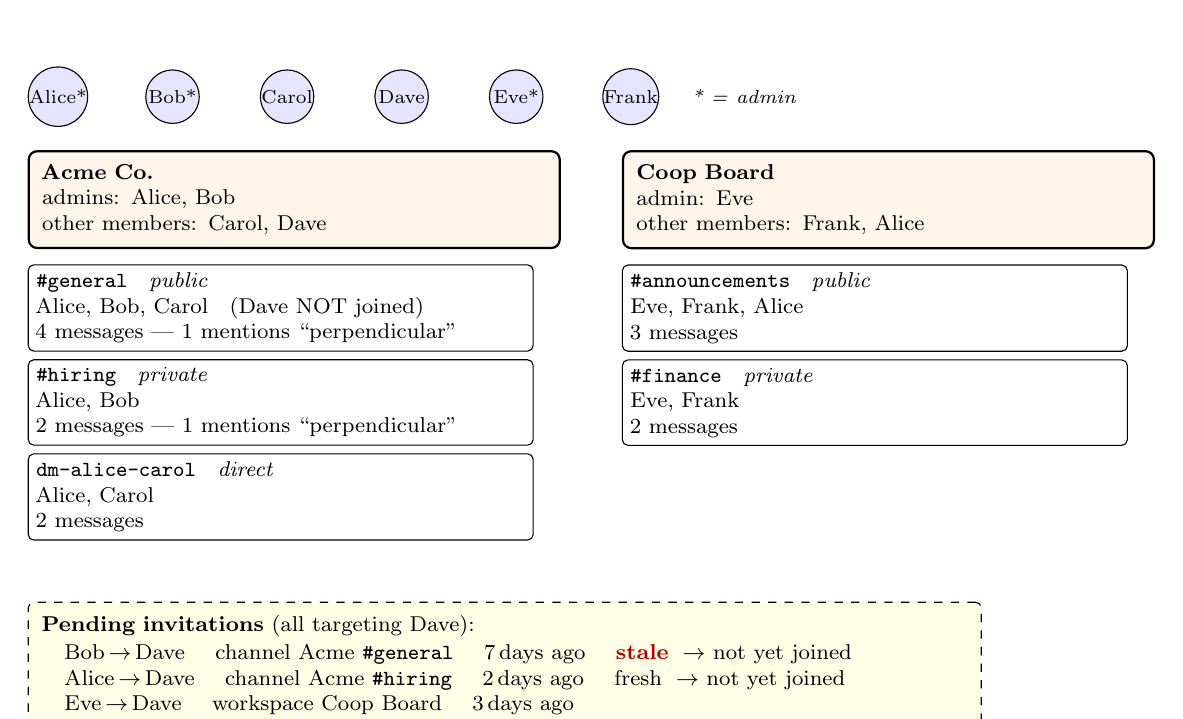
\begin{tikzpicture}[scale=0.97, transform shape,
  font=\footnotesize,
  ws/.style={rectangle, draw, thick, rounded corners=3pt,
             fill=orange!8, inner sep=5pt, align=left},
  ch/.style={rectangle, draw, thin, rounded corners=2pt,
             fill=white, inner sep=3pt, align=left, text width=6.4cm},
  invbox/.style={rectangle, draw, dashed, rounded corners=2pt,
             fill=yellow!10, inner sep=5pt, align=left, text width=\linewidth},
  user/.style={circle, draw, fill=blue!10, minimum size=0.7cm,
             inner sep=0pt, font=\scriptsize},
]

% ---- Users row ----
\node[user] (alice) at (0, 0)   {Alice*};
\node[user] (bob)   at (1.5, 0) {Bob*};
\node[user] (carol) at (3.0, 0) {Carol};
\node[user] (dave)  at (4.5, 0) {Dave};
\node[user] (eve)   at (6.0, 0) {Eve*};
\node[user] (frank) at (7.5, 0) {Frank};
\node[font=\scriptsize, right=0.3cm of frank] {\textit{* = admin}};

% ---- Acme workspace ----
\node[ws, below=0.7cm of alice.west, anchor=north west, text width=6.6cm] (acme) {%
  \textbf{Acme Co.}\\
  admins: Alice, Bob\\
  other members: Carol, Dave
};
\node[ch, below=2mm of acme.south west, anchor=north west] (gen) {%
  \texttt{\#general} \; \emph{public}\\
  Alice, Bob, Carol \; (Dave NOT joined) \\
  4 messages --- 1 mentions ``perpendicular''
};
\node[ch, below=1mm of gen.south west, anchor=north west] (hir) {%
  \texttt{\#hiring} \; \emph{private}\\
  Alice, Bob \\
  2 messages --- 1 mentions ``perpendicular''
};
\node[ch, below=1mm of hir.south west, anchor=north west] (dm) {%
  \texttt{dm-alice-carol} \; \emph{direct}\\
  Alice, Carol \\
  2 messages
};

% ---- Coop Board workspace ----
\node[ws, right=0.8cm of acme.north east, anchor=north west, text width=6.6cm] (coop) {%
  \textbf{Coop Board}\\
  admin: Eve\\
  other members: Frank, Alice
};
\node[ch, below=2mm of coop.south west, anchor=north west] (ann) {%
  \texttt{\#announcements} \; \emph{public}\\
  Eve, Frank, Alice \\
  3 messages
};
\node[ch, below=1mm of ann.south west, anchor=north west] (fin) {%
  \texttt{\#finance} \; \emph{private}\\
  Eve, Frank \\
  2 messages
};

% ---- Invitations (pending) ----
\node[invbox, below=0.8cm of dm.south west, anchor=north west] (inv) {%
  \textbf{Pending invitations} (all targeting Dave):\\[1pt]
  \hspace*{1em}Bob\,$\to$\,Dave \quad channel Acme \texttt{\#general}
      \quad 7\,days ago \quad \textbf{\textcolor{red!70!black}{stale}}
      \;$\rightarrow$ not yet joined \\
  \hspace*{1em}Alice\,$\to$\,Dave \quad channel Acme \texttt{\#hiring}
      \quad 2\,days ago \quad fresh
      \;$\rightarrow$ not yet joined \\
  \hspace*{1em}Eve\,$\to$\,Dave \quad workspace Coop Board
      \quad 3\,days ago
};

\end{tikzpicture}
\end{figure}

\subsection*{Query Testing}
After loading the sample data, the queries in part (c) were executed against
the populated database. The observed results are shown below.

\noindent\textbf{(1) Create a new user account}

This test inserts a new user named Grace and returns the generated
\texttt{user\_id}.

\noindent\textbf{Query.}
\begin{lstlisting}
INSERT INTO users (email, username, nickname, password_hash)
VALUES ('grace@acme.com', 'grace', 'Grace', 'hash_grace')
RETURNING user_id;
\end{lstlisting}

\noindent\textbf{Result.}
\begin{lstlisting}[style=result]
user_id
-------
7
(1 row)

INSERT 0 1
\end{lstlisting}

\noindent\textbf{(2) Create a public channel (with authorization check)}

This test first lets Alice (\texttt{user\_id}=1), who is a member of Acme
(\texttt{workspace\_id}=1), create a new public channel \texttt{\#random}; it
then adds her to \texttt{channel\_members}. The second test lets Eve
(\texttt{user\_id}=5) attempt the same operation in Acme
(\texttt{workspace\_id}=1), but since she is not a member of that workspace,
the guarded insert returns no rows.

\noindent\textbf{Query.}
\begin{lstlisting}
-- Test A: Alice, who is an Acme member, creates #random.
INSERT INTO channels (workspace_id, name, type, created_by)
SELECT 1, '#random', 'public', 1
WHERE EXISTS (
    SELECT 1 FROM workspace_members
    WHERE workspace_id = 1 AND user_id = 1
)
RETURNING channel_id;

INSERT INTO channel_members (channel_id, user_id)
VALUES (6, 1);

-- Test B: Eve tries to create a channel in Acme, but she is not a member.
INSERT INTO channels (workspace_id, name, type, created_by)
SELECT 1, '#eve-unauthorized', 'public', 5
WHERE EXISTS (
    SELECT 1 FROM workspace_members
    WHERE workspace_id = 1 AND user_id = 5
)
RETURNING channel_id;
\end{lstlisting}

\noindent\textbf{Result.}

\noindent{\footnotesize\textbf{Test A: Alice, who is an Acme member, creates \texttt{\#random}.}}
\begin{lstlisting}[style=result]
channel_id
----------
6
(1 row)

INSERT 0 1
INSERT 0 1
\end{lstlisting}

\noindent{\footnotesize\textbf{Test B: Eve tries to create a channel in Acme, but she is not a member.}}
\begin{lstlisting}[style=result]
channel_id
----------
(0 rows)

INSERT 0 0
\end{lstlisting}

\noindent\textbf{(3) For each workspace, list all administrators}

This query joins \texttt{workspaces}, \texttt{workspace\_members}, and
\texttt{users} to list every administrator in each workspace.

\noindent\textbf{Query.}
\begin{lstlisting}
SELECT w.workspace_id, w.name AS workspace, u.username AS administrator
FROM   workspaces w
JOIN   workspace_members wm ON wm.workspace_id = w.workspace_id
JOIN   users u              ON u.user_id       = wm.user_id
WHERE  wm.is_admin = TRUE
ORDER BY w.workspace_id, u.username;
\end{lstlisting}

\noindent\textbf{Result.}
\begin{lstlisting}[style=result]
workspace_id | workspace  | administrator
-------------|------------|--------------
1            | Acme Co.   | alice
1            | Acme Co.   | bob
2            | Coop Board | eve
(3 rows)
\end{lstlisting}

\noindent\textbf{(4) Per public channel: \# invitees invited $>$5 days ago, not yet joined}

This query counts, for each public channel in Acme
(\texttt{workspace\_id}=1), the pending invitations that are older than five
days and whose invitees still do not appear in \texttt{channel\_members}.

\noindent\textbf{Query.}
\begin{lstlisting}
SELECT c.channel_id, c.name,
       COUNT(ci.invitee_user_id) FILTER (WHERE cm.user_id IS NULL)
       AS stale_unjoined_invites
FROM   channels c
LEFT   JOIN channel_invitations ci
       ON ci.channel_id = c.channel_id
      AND ci.invited_at < CURRENT_TIMESTAMP - INTERVAL '5 days'
LEFT   JOIN channel_members cm
       ON cm.channel_id = ci.channel_id AND cm.user_id = ci.invitee_user_id
WHERE  c.workspace_id = 1
  AND  c.type = 'public'
GROUP BY c.channel_id, c.name
ORDER BY c.name;
\end{lstlisting}

\noindent\textbf{Result.}
\begin{lstlisting}[style=result]
channel_id |   name   | stale_unjoined_invites
-----------+----------+------------------------
1          | #general |                      1
6          | #random  |                      0
(2 rows)
\end{lstlisting}

\noindent\textbf{(5) All messages in a channel, chronological order}

This test retrieves all messages in Acme \texttt{\#general}
(\texttt{channel\_id}=1) and orders them by \texttt{posted\_at} and then by
\texttt{message\_id}.

\noindent\textbf{Query.}
\begin{lstlisting}
SELECT m.message_id, m.posted_at, u.username, m.body
FROM   messages m
JOIN   users u ON u.user_id = m.sender_user_id
WHERE  m.channel_id = 1
ORDER BY m.posted_at ASC, m.message_id ASC;
\end{lstlisting}

\noindent\textbf{Result.}
\begin{lstlisting}[style=result]
message_id |         posted_at          | username |                          body
-----------+----------------------------+----------+---------------------------------------------------------
1          | 2026-04-14 21:26:56.771839 | alice    | Welcome to Acme #general!
2          | 2026-04-16 21:26:56.771839 | bob      | Standup notes will be posted here daily.
3          | 2026-04-18 21:26:56.771839 | carol    | Quick geometry question: are these lines perpendicular?
4          | 2026-04-19 21:26:56.771839 | alice    | Let's meet tomorrow at 10am.
(4 rows)
\end{lstlisting}

\noindent\textbf{(6) All messages posted by a given user}

This query lists all messages posted by Alice (\texttt{user\_id}=1) across all
channels and workspaces, ordered from newest to oldest.

\noindent\textbf{Query.}
\begin{lstlisting}
SELECT m.message_id, w.name AS workspace, c.name AS channel,
       m.posted_at, m.body
FROM   messages m
JOIN   channels   c ON c.channel_id   = m.channel_id
JOIN   workspaces w ON w.workspace_id = c.workspace_id
WHERE  m.sender_user_id = 1
ORDER BY m.posted_at DESC;
\end{lstlisting}

\noindent\textbf{Result.}
\begin{lstlisting}[style=result]
message_id | workspace  |    channel     |         posted_at          |                   body
-----------+------------+----------------+----------------------------+-------------------------------------------
4          | Acme Co.   | #general       | 2026-04-19 21:26:56.771839 | Let's meet tomorrow at 10am.
11         | Coop Board | #announcements | 2026-04-17 21:26:56.771839 | Could someone share last month's minutes?
5          | Acme Co.   | #hiring        | 2026-04-15 21:26:56.771839 | Candidate feedback for the backend role.
1          | Acme Co.   | #general       | 2026-04-14 21:26:56.771839 | Welcome to Acme #general!
7          | Acme Co.   | dm-alice-carol | 2026-04-11 21:26:56.771839 | Hey Carol, got a minute?
(5 rows)
\end{lstlisting}

\noindent\textbf{(7) Accessible messages containing ``perpendicular''}

This test checks accessibility for three different users: Alice
(\texttt{user\_id}=1), Carol (\texttt{user\_id}=3), and Dave
(\texttt{user\_id}=4). Alice is a member of both Acme channels that contain the
keyword, Carol is only a member of \texttt{\#general}, and Dave is an Acme
workspace member but not a member of any Acme channel.

\noindent\textbf{Query.}
\begin{lstlisting}
-- Test A: Alice (user_id = 1)
SELECT m.message_id, w.name AS workspace, c.name AS channel,
       u.username AS author, m.posted_at, m.body
FROM   messages m
JOIN   channels         c  ON c.channel_id    = m.channel_id
JOIN   workspaces       w  ON w.workspace_id  = c.workspace_id
JOIN   users            u  ON u.user_id       = m.sender_user_id
JOIN   channel_members  cm ON cm.channel_id   = c.channel_id
                          AND cm.user_id      = 1
JOIN   workspace_members wm ON wm.workspace_id = w.workspace_id
                           AND wm.user_id      = 1
WHERE  m.body ILIKE '%perpendicular%'
ORDER BY m.posted_at DESC;

-- Test B: Carol (user_id = 3)
SELECT m.message_id, w.name AS workspace, c.name AS channel,
       u.username AS author, m.posted_at, m.body
FROM   messages m
JOIN   channels         c  ON c.channel_id    = m.channel_id
JOIN   workspaces       w  ON w.workspace_id  = c.workspace_id
JOIN   users            u  ON u.user_id       = m.sender_user_id
JOIN   channel_members  cm ON cm.channel_id   = c.channel_id
                          AND cm.user_id      = 3
JOIN   workspace_members wm ON wm.workspace_id = w.workspace_id
                           AND wm.user_id      = 3
WHERE  m.body ILIKE '%perpendicular%'
ORDER BY m.posted_at DESC;

-- Test C: Dave (user_id = 4)
SELECT m.message_id, w.name AS workspace, c.name AS channel,
       u.username AS author, m.posted_at, m.body
FROM   messages m
JOIN   channels         c  ON c.channel_id    = m.channel_id
JOIN   workspaces       w  ON w.workspace_id  = c.workspace_id
JOIN   users            u  ON u.user_id       = m.sender_user_id
JOIN   channel_members  cm ON cm.channel_id   = c.channel_id
                          AND cm.user_id      = 4
JOIN   workspace_members wm ON wm.workspace_id = w.workspace_id
                           AND wm.user_id      = 4
WHERE  m.body ILIKE '%perpendicular%'
ORDER BY m.posted_at DESC;
\end{lstlisting}

\noindent\textbf{Result.}

\noindent{\footnotesize\textbf{Test A: Alice (user\_id = 1).}}
\begin{lstlisting}[style=result]
message_id | workspace | channel  | author |         posted_at          |                             body
-----------+-----------+----------+--------+----------------------------+--------------------------------------------------------------
3          | Acme Co.  | #general | carol  | 2026-04-18 21:26:56.771839 | Quick geometry question: are these lines perpendicular?
6          | Acme Co.  | #hiring  | bob    | 2026-04-17 21:26:56.771839 | Their system-design answer had two perpendicular approaches.
(2 rows)
\end{lstlisting}

\noindent{\footnotesize\textbf{Test B: Carol (user\_id = 3).}}
\begin{lstlisting}[style=result]
message_id | workspace | channel  | author |         posted_at          |                          body
-----------+-----------+----------+--------+----------------------------+---------------------------------------------------------
3          | Acme Co.  | #general | carol  | 2026-04-18 21:26:56.771839 | Quick geometry question: are these lines perpendicular?
(1 row)
\end{lstlisting}

\noindent{\footnotesize\textbf{Test C: Dave (user\_id = 4).}}
\begin{lstlisting}[style=result]
message_id | workspace | channel | author | posted_at | body
-----------+-----------+---------+--------+-----------+------
(0 rows)
\end{lstlisting}

\end{document}
